\documentclass[10 pt]{article}

\usepackage{fontspec}
\defaultfontfeatures{Mapping=tex-text}
\setmainfont{Minion Pro}

%\usepackage{graphicx}
%\usepackage{fullpage}

\usepackage{lastpage, fancyhdr}
\pagestyle{fancy}
\lhead{Scott O'Connor}
\chead{Phil 234} 
\rhead{\emph{Meno}}
\lfoot{}
\cfoot{\thepage\space of \pageref{LastPage}} 
\rfoot{}

\thispagestyle{empty}


\begin{document}
\author{Phil 234}
\title{\emph{Meno}}
\maketitle

\subsection{Overview}

Structure of dialog.

\section*{The priority of definition}

\noindent If you don't know what something is, you can't know what qualities it has---i.e. you can't know anything else about it (71b3-4)
\vspace*{2mm}

\noindent In other words, knowing whether \emph{X} is \emph{F} is epistemically \emph{posterior} to knowing what \emph{X} is

\begin{itemize}\item{So, knowing what virtue is is a necessary condition for knowing whether virtue is teachable. Thus, Socrates and Meno turn their attention to determining what virtue is.}\end{itemize}

\noindent What conception of knowledge might make this plausible?

\section*{The paradox of inquiry}

\noindent Meno's version: He asks, first, ``How will you look for it [the nature of virtue] when you do not know at all what it is?'' And then presents something like a dilemma:
\vspace*{2mm}

\noindent Grube translation of 80d5-7: ``How will you aim to search for something you do not know at all? If you should meet with it, how will you know that this is the thing that you did not know?''
\vspace*{2mm}

\noindent Alternative translation: ``Which among the things you do not know [to be virtue] will you put before you to investigate? Or, if you happened to encounter it [the nature of virtue], how will you know that this is it, that thing which you did not know?''
\vspace*{2mm}

\noindent Socrates' version
\begin{itemize}\item{[1] Inquiry is impossible}\item{[2] If X knows, there is no point in searching (since X knows it already)}\item{[3] If X doesn't know, X cannot search (since X doesn't know what to search for)}\begin{itemize}\item{What suppressed premise is necessary to make [2], [3]$\rightarrow$ [1] a valid argument?}\end{itemize}\end{itemize}

\noindent What is the relationship between Meno's version and Socrates' version?

\section*{Socrates' response: Recollection and the Exchange with Meno's slave}

\noindent Plato clearly takes the paradox seriously, but which premise of the dilemma does he reject?
\vspace*{2mm}

\begin{itemize}\item{[R] Learning is recollection---which seems to reject [2]: you \emph{already} knew and \emph{later} recollect}\item{[E] The elenchus of the slave---which seems to reject [3]: the slave didn't know and now does (or will after further questioning)}\item{Perhaps he rejects [2] and [3]: There is a sense in which you can know (i.e. latently) but still have successful inquiry (by recollecting) (i.e. 2 is false) and there is a sense in which you don't know (i.e. explicitly) and can still have successful inquiry (i.e. in an exchange such as the one with Meno's slave)}\end{itemize}

\noindent S claims that the slave:
\begin{itemize}\item{[A] Has not learned geometry before}\item{[B] Was not taught it by him in this episode--so the slave didn't \emph{learn} it then either}\item{[C] And yet \emph{will} know it through further questioning}\end{itemize}

\noindent Re [B]: S claims that his questions merely elicit the slave's opinions. S did use the elenctic method---he asks misleading questions sometimes; he gets the slave to claim knowledge and then to confess \emph{aporia}; thereafter the slave gets it right by applying his own reasoning, not by bowing to S's authority.
\vspace*{2mm}

\noindent Perhaps, then, [R] supports [E]. We need some explanation of why the slave, through his discussion with S, will reliably \emph{reject} false beliefs and \emph{accept} true beliefs. Perhaps S thinks this is possible because the slave (like everyone) once knew (in a disembodied state) but forgot, and hence can recognize the truth, and so reject the false.
\vspace*{2mm}

\noindent Additional question: Even if we grant [A]-[C] do we have to think that the slave has recollected knowledge? What alternative explanations for the success of the slave's discussion might we consider?

\section*{The scope of recollection}

\noindent What kinds of truths does S think we can recollect?

\begin{itemize}\item{He clealy allows geometrical truths (and so mathematical truths generally?). He should allow ethical truths (including truths about value) (otherwise the unity of the dialogue would be in jeopardy). He also suggests nature ``as a whole''?---What could that mean?}\item{What about empirical truths?}\end{itemize}

\section*{Recollection revisited}

\noindent [1] The slave is said to have no geometrical knowledge before the discussion (85e)
\vspace*{2mm}

\noindent [2] S claims that he has not taught the slave anything during their discussion
\begin{itemize}\item{S is probably working with a conception of ``teaching'' on which for S to teach X that P would be for X to come to believe that P \emph{only because} S tells X that P}\end{itemize}

\noindent [3] But, by the end of the discussion, the slave has the opinion that the double-area square comes to be from the diagonal of the original square

\begin{itemize}\item{So, given [2], S asks where that opinion came from}\item{S claims that it must have been, in some sense, in the slave already (85c)}\end{itemize}

\noindent [4] S claims that the slave, at the end of the discussion, does not yet have \emph{epist\^{e}m\^{e}} of the geometrical fact, but that the slave \emph{will} acquire it through further questioning (85c7-d4)
\vspace*{2mm}

\noindent [5] Since that further questioning will not violate [2], S concludes that the slave will acquire the knowledge ``from himself by himself''
\vspace*{2mm}

\noindent [6] The phenomenon described in [5] is claimed to be an instance of ``recollection'' (\emph{anamn\^{e}sis})
\vspace*{2mm}

\noindent So, S takes himself to have answered the paradox of inquiry by showing that the slave can go from a state of not having \emph{epist\^{e}m\^{e}} (at least, not explicitly) to a state of having \emph{epist\^{e}m\^{e}} (i.e. explicitly). And, he maintains that it is because the slave once knew, then forgot, and through questioning can be made to recollect, that successful inquiry is possible. So, is it because those who don't know have true opinions which they can systematize in some way that successful inquiry is possible?
\vspace*{2mm}

\noindent Important question: Even if we grant [1]-[4] do we have to think that the slave has (or, will have) recollected knowledge? What alternative explanations for the success of the slave's discussion might we consider?

\section*{The scope of recollection}

\noindent What kinds of truths does S think we can recollect?

\begin{itemize}\item{He clearly allows geometrical truths (and so mathematical truths generally?). He should allow ethical truths (including truths about value) (otherwise the unity of the dialogue would be in jeopardy). He also suggests nature ``as a whole''?---What could that mean?}\item{What about empirical truths?}\end{itemize}

\section*{Is virtue knowledge/understanding?}

\noindent After the exchange, M insists that S address whether virtue is teachable, despite S's demand to determine what virtue is first
\vspace*{2mm}

\noindent S again refuses to address that question directly, but instead notes that if virtue is knowledge, then virtue will be teachable (and if virtue is not knowledge, it will not be teachable)
\vspace*{2mm}

\noindent So he then turns his attention to the question whether virtue is knowledge, considering arguments for and against
\begin{itemize}\item{The main \emph{pro} argument is that, since virtue is beneficial, and all actions guided by knowledge turn out well, virtue must be knowledge}\end{itemize}

\section*{The difference between true belief/opinion and knowledge/understanding}

\noindent S maintains that they were right to say that actions guided by knowledge always turn out correctly, BUT
\vspace*{2mm}

\noindent They were wrong to say that \emph{only} actions guided by knowledge turn out correctly---actions guided by true opinion (\emph{doxa}) also turn out correctly

\begin{itemize}\item{The example of the ``Road to Larissa'' (97a5-c2) is supposed to show this}\end{itemize}

\noindent This leads M to ask ``why knowledge (\emph{epist\^{e}m\^{e}}) is prized far more highly than right opinion, and why they are different'' (97d1-2)
\vspace*{2mm}

\noindent S answers that right opinion is ``upgraded'' into knowledge by a ``giving an account of the reason why'' (i.e. by working out the explanation of the relevant fact) which ``ties'' the opinion to the soul. Knowledge is more valuable because it remains in place.
\vspace*{2mm}

\noindent Question: What has \emph{not} been done in the discussion with the slave such that further questioning could lead the slave to work out the explanation of the geometrical theorem?
\vspace*{2mm}

\section*{How natures can play an explanatory role}

\noindent Euclid's \emph{Elements} Book 1, Proposition 34: In parallelogrammic figures the opposite sides and angles are equal to one another, and \emph{a diagonal cuts them in half}
\vspace*{2mm}

\noindent And, [F1] since the point A is the center of the circle CDB, [F2] AC is equal to AB.

\begin{figure}[h!]
\centering
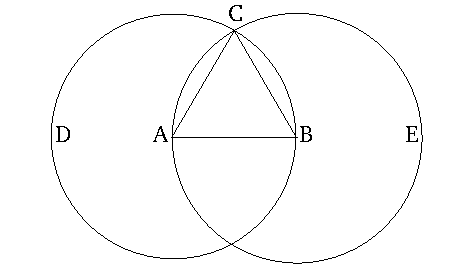
\includegraphics[scale=0.7]{circle}
%\caption{}
%\label{fig:prop 34}
\end{figure}

\noindent Definition of Circle: A Circle is a plane figure contained by one line, such that all of the straight-lines falling upon it from one point among those lying within the figure are equal to one another

\end{document}

